\documentclass[]{spie}
	\usepackage{graphicx}
	\usepackage{float}
	\usepackage{color}
	\usepackage{colortbl}
	\title {Mipsilon: A single-cycle simulation\\of the MIPS architecture }
	\author {V. Valadez\footnote[1]{ \ valadev@cc.wwu.edu}  \\
          Computer Science, Western Washington Univ.\\
	Belligham, WA 98225
	}
\begin{document}
	\maketitle

\begin{abstract}
Mipsilon is a visual simulation of a single-cycle implementation of the MIPS architecture. It is intended to 
be used as a tool for learning how basic MIPS instructions are executed rather than a perfect simulation of the
architecture. In this architecture only a subset of the MIPS instructions are actually implemented: 
{\bf add, addi, sub, and, or, slt, beq, j, jr, jal}. This small subset is sufficient enough to demonstrate
common control structures and procedure calls in a MIPS assembly program.
\end{abstract}

%\section{INTRODUCTION}
%\cite{Hennessy98}
%\cite{Wilson02}

\section{MATERIALS AND METHODS}
The Mipsilon program was developed using the model/view design pattern.
The core components, described in section \ref{sec:SystemOverview}, work entirely independent from the rest of the program. 
Java's Swing package was used as a layer to wrap the core in a friendly user interface.


\section{SYSTEM OVERVIEW}
\label{sec:SystemOverview}

\subsection{CPU}
The CPU component encapsulates the CPU sub-components and provides high level operations for executing instructions.
This component is responsible for creating and managing the Control Unit, ALU, ALU Control, and Register File components. It also
manages references to Text Memory and Data Memory that are created outside of the CPU component.

High level operations of the CPU component are described:

\begin{itemize}
	\item The {\bf reset} operation will reset all the registers
	in the Register File, and reset the program counter to zero.
	\item The {\bf execute} operation retrieves the instruction that's stored in the Text Memory
	at the address of the current program counter, execute the instruction, and adjust the program counter
	accordingly.
\end{itemize}

\subsection{Control Unit}
The Control Unit is a very simple component. It consists of a 6-bit input and nine 1-bit outputs that
control data paths and other components plus one 2-bit output that provides one of the inputs to the ALU Control component.

\begin{table}[H]
	\begin{center}
	\begin{tabular}{|c|c|c|c|c|c|c|}
		\hline
		\rowcolor[gray]{.9} {\bf Op Code} & {\bf ControlOp} & {\bf AluSrc} & {\bf Jump} & {\bf Branch}  & {\bf RegDst} & {\bf MemToReg} \\[6pt]
		\hline
		\rowcolor[gray]{.9}  { } &        &{ \bf MemWrite } & {\bf MemRead}& {\bf RegWrite}& {\bf Link} & { } \\[6pt]
		\hline
					${\tt 000000_{\rm binary}}$ & ${\tt 10_{\rm binary}}$ &{\tt 0}&{\tt 0}&{\tt 0}&{\tt 1}&{\tt 0}\\
		                             R-type  &          &{\tt 0}&{\tt 0}&{\tt 1}&{\tt 0}&       \\
		\hline
		                        ${\tt 100011_{\rm binary}}$ & ${\tt 00_{\rm binary}}$ &{\tt 1}&{\tt 0}&{\tt 0}&{\tt 0}&{\tt 1}\\
		                          lw   &          &{\tt 0}&{\tt 1}&{\tt 1}&{\tt 0}&       \\
		\hline
					${\tt 101011_{\rm binary}}$ & ${\tt 00_{\rm binary}}$ &{\tt 1}&{\tt 0}&{\tt 0}&{\tt 0}&{\tt 0}\\
		                          sw         &          &{\tt 0}&{\tt 1}&{\tt 0}&{\tt 0}&       \\
		\hline
					${\tt 000100_{\rm binary}}$ & ${\tt 01_{\rm binary}}$ &{\tt 0}&{\tt 0}&{\tt 1}&{\tt 0}&{\tt 0}\\
		                           beq       &          &{\tt 0}&{\tt 0}&{\tt 0}&{\tt 0}&       \\
		\hline
					${\tt 000010_{\rm binary}}$ & ${\tt 00_{\rm binary}}$ &{\tt 0}&{\tt 1}&{\tt 0}&{\tt 0}&{\tt 0}\\
		                           j         &          &{\tt 0}&{\tt 0}&{\tt 0}&{\tt 0}&       \\
		\hline
					${\tt 000011_{\rm binary}}$ & ${\tt 00_{\rm binary}}$ &{\tt 0}&{\tt 1}&{\tt 0}&{\tt 0}&{\tt 0}\\
		                            jal      &          &{\tt 0}&{\tt 0}&{\tt 0}&{\tt 1}&       \\
		\hline
					${\tt 001000}_{\rm binary}$ & ${\tt 00_{\rm binary}}$ &{\tt 1}&{\tt 0}&{\tt 0}&{\tt 0}&{\tt 0}\\
		                             addi    &          &{\tt 0}&{\tt 0}&{\tt 1}&{\tt 0}&       \\
		\hline
	\end{tabular}
	\end {center}
	\caption{\label{tab:ControlUnit} Control Unit implementation}
\end{table}

\subsection{ALU Control}
The ALU Control component consists of two inputs and two outputs. The inputs consist of a 2-bit input connected to the Control Unit
and a 6-bit input that comes from bits {\tt [5-0]} of the instruction, its Funct field. The two outputs are
a 3-bit output that controls the ALU directly and a 1-bit output used for the jr instruction.
          
     
\begin{table}[H]
	\begin{center}
	\begin{tabular}{|c|c||c|c|c|}
		\hline
		\rowcolor[gray]{.9} {\bf ControlOp} &{\bf Funct field} & {\bf Jr} & {\bf ALU Control} & {\bf ALU } \\ [12pt]
		\hline
		${\tt 00_{\rm binary}}$ & -                         & {\tt 0} & ${\tt 010_{\rm binary}}$ &{\bf add} \\
		${\tt 01_{\rm binary}}$ & -                         & {\tt 0} & ${\tt 110_{\rm binary}}$ &{\bf sub} \\
		${\tt 10_{\rm binary}}$ & ${\tt 100000_{\rm binary}}$ & {\tt 0} & ${\tt 010_{\rm binary}}$ &{\bf add} \\
		${\tt 10_{\rm binary}}$ & ${\tt 100010_{\rm binary}}$ & {\tt 0} & ${\tt 110_{\rm binary}}$ &{\bf sub} \\
		${\tt 10_{\rm binary}}$ & ${\tt 100100_{\rm binary}}$ & {\tt 0} & ${\tt 000_{\rm binary}}$ &{\bf and} \\
		${\tt 10_{\rm binary}}$ & ${\tt 100101_{\rm binary}}$ & {\tt 0} & ${\tt 001_{\rm binary}}$ &{\bf or} \\
		${\tt 10_{\rm binary}}$ & ${\tt 101010_{\rm binary}}$ & {\tt 0} & ${\tt 111_{\rm binary}}$ &{\bf slt} \\
		${\tt 10_{\rm binary}}$ & ${\tt 001000_{\rm binary}}$ & {\tt 1} & - & - \\
		\hline
	\end{tabular}
	\end {center}
	\caption{\label{tab:ALUControl} Currently supported ALU functions}
\end{table}

\subsection{ALU}
This simple ALU consists of two 32-bit inputs A and B, one 3-bit control input, one 32-bit result output, and
a 1-bit zero control line which is asserted when the result of the operation is zero. Out of the eight operations
possible with a 3-bit control input only five operations are actually valid in this implementation.
The five operations that are valid for this ALU are listed in Table \ref{tab:ALU}.

\begin{table}[H]
	\begin{center}
	\begin{tabular}{|p{1.0in}|p{1.0in}|p{3.2in}|}
		\hline
		\rowcolor[gray]{.9}{\bf Operation} &{\bf Control}  & {\bf Description} \\
		\rowcolor[gray]{.9} { } &{ } & { }   \\
		\hline
		and & ${\tt 000_{\rm binary}}$ & Provides a logical and of two 32-bit integers \\
		\hline
		or & ${\tt 001_{\rm binary}}$ & Provides a logical or of two 32-bit integers \\
		\hline
		add & ${\tt 010_{\rm binary}}$ & Provides signed addition of two 32-bit integers \\
		\hline
		sub & ${\tt 110_{\rm binary}}$ & Provides signed subtraction of two 32-bit integers \\
		\hline
		slt & ${\tt 111_{\rm binary}}$ & Subtracts two 32-bit numbers and sets the output to 1 if the result is
		negative and 0 if the result is positive \\
		\hline
	\end{tabular}
	\end {center}
	\caption{\label{tab:ALU} Currently supported ALU functions}
\end{table}

\subsection{Register File}
The Register component simply holds the data that's stored in the registers. The CPU component interacts with the 
Register component through an interface similar to the graphical representation. ReadRegister1, ReadRegister2, and
the WriteRegister are set according to the instruction. Register values are read from RegisterData1, RegisterData2. 
The write operation will fill the WriteRegister with the data that's in WriteData. The link operation will copy the
value of the program counter into register 31.

\subsection{Memory}
The memory component provides a mapping from a 32-bit integer address to a byte. In other words, it is byte addressable, however only 32-bit 
words are read or written at a time. Big Endian order is assumed in this implementation. 


\subsection{Assembler}

\subsubsection{Assembler directives and literals}
The {\tt .text} and {\tt .data} directives separate the two memory segments. All instructions or data definitions must
be defined within their respective environment in the source file. Only one text and one data segment can be defined in
one source file. No attempt is made to do any sort of linking with other programs or modules. Both text and data segments are
assumed to start at offset {\tt 0x00000000}. Since the Text memory is separate from the Data memory in this simulation this
won't cause conflicts of any kind.

The assembler understands three types of integer literals: hexadecimal, octal, and decimal. A hexadecimal number is preceded by
{\tt `0x'}, an octal numer is preceded by {\tt `0'}, all other numbers are assumed to be decimal. String literals are enclosed in
double quotes. 

\subsubsection{Text segment}
The only instructions the assembler will recognize are the instructions
implemented by the simulator. The {\bf la} instruction is the only pseudo instruction currently implemented.

\subsubsection{Data segment}
The data processing component of the assembler can understand six types of data: {\bf space}, {\bf byte}, {\bf half}, {\bf word}, {\bf ascii} and {\bf asciiz}.
No attepmt to align data is made. It is the responsibility of the programmer to properly align the data.

\section{DEMONSTRATION}
When the application is first started the text and data memories are empty. A program can either be loaded from 
a source file on the local file system or by loading one of the sample programs included with the application. These sample
programs can be found under the Programs menu.

Once a progam is successfully assembled and loaded into memory the Text, Disassembly, and Data windows will be updated.
Figures \ref{fig:Text} and \ref{fig:Disassembly} show the Text and Disassembly windows after a program has been loaded.
Figure \ref{fig:Data} shows the Data window after a program has been loaded. Use the tool bar to single-step through the program.
The stop button will perform a ``soft'' reset: the program counter and registers are reset to zero.

\begin{center}
\begin{figure}[H]	
	\begin{center}
	\begin{minipage}[H]{2.4in}
		\begin{center}
			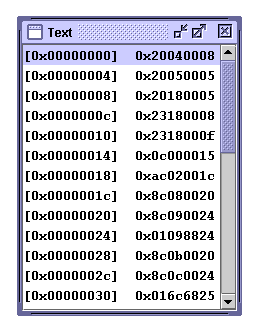
\includegraphics{graphics/TextWindow.eps}
		\end{center}
		
		\caption{\label{fig:Text} Text Window}
		
	\end{minipage}
	\ 
	\begin{minipage}[H]{2.7in}
		\begin{center}
			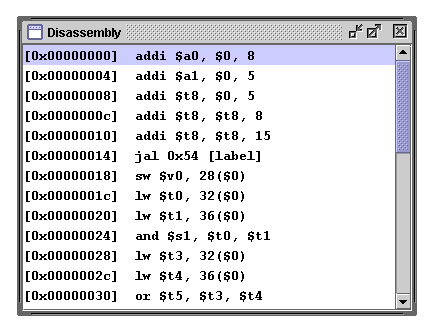
\includegraphics{graphics/DisassemblyWindow.eps}			
		\end{center}
		\caption{\label{fig:Disassembly}Disassembly Window}
	\end{minipage}	
	\end{center}
\end{figure}
\end{center}

\begin{center}
\begin{figure}[H]	
	\begin{center}
	\begin{minipage}{2.4in}
		\begin{center}
			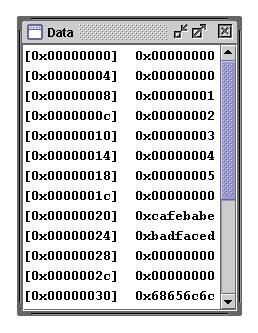
\includegraphics{graphics/DataWindow.eps}			
		\end{center}		
		\caption{\label{fig:Data} Data Window}	
	\end{minipage}
	\ 	
	\begin{minipage}{2.7in}
		\begin{center}
			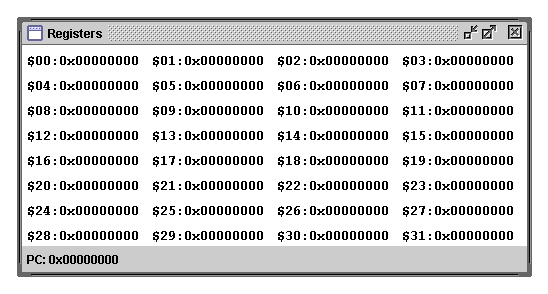
\includegraphics{graphics/RegistersWindow.eps}			
		\end{center}
		\vspace{17pt}
		\caption{\label{fig:Registers}Registers Window}
	\end{minipage}	
	\end{center}	
\end{figure}
\end{center}

Figue \ref{fig:Simulator} shows the CPU simulator window. It is a graphical representation of the data and control lines after
an instruction has executed.  

\begin{figure}[H]
	\begin{center}
		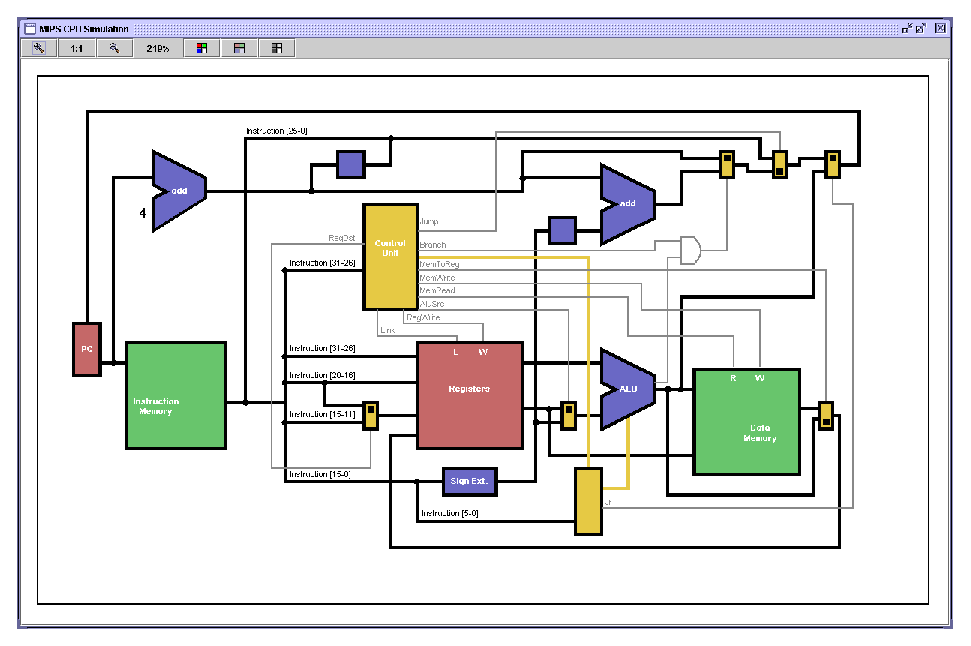
\includegraphics{graphics/Simulator.eps}
	\end{center}
	\caption{\label{fig:Simulator} Simulator Window}
\end{figure}

%\bibliography{report}   %>>>> bibliography data in report.bib
%\bibliographystyle{spiebib}
\begin{thebibliography}{1}

\bibitem{Hennessy98}
J.~L. Hennessy and D.~A. Patterson, {\em Computer Organization and Design
  Second Edition}, Morgan Kaufman, San Francisco, California, 1998.

\bibitem{Wilson}
G.~R. Wilson, {\em Embedded Systems and Computer Architecture}, Newnes, Oxford,
  2002.

\end{thebibliography}

\section*{APPENDIX A}
\subsection*{A.1 Sample Programs}

\subsubsection*{A.1.1 sample1.mips}
\begin{center}
\begin{verbatim}
##############################
# sample1.mips
#
# Author: Victor Valadez
# Date:   March 6, 2004
# 
# This sample program demonstrates the use
# of a procedure call.
# 
#############################

        .text   

main:   
        la      $a0,  arr       # load the address of the array
        addi    $a1,   $0, 5    # Set array size
        jal SumArray            # Execute the function
                        
        sw      $v0,    result  # Save the result into memory
        
        j main                  # Jump back to main

##############################
#
# SumArray
# sums all numbers in a word array
# input: 
#        $a0 - the array to sum
#        $a1 - the size of the array
#output:
#        $v0 - the sum
SumArray:
        add  $t0, $0,   $a0      # Copy the array pointer
        add  $t1, $0,   $a1      # Copy the array size
        addi $t1, $t1,   -1      # Loop counter = array size - 1.
        add  $v0, $0,   $0       # Initialize return value
SumArrayLoop:   
        slt  $t2, $0,   $t1        
        beq  $0,  $t2,  SumArrayExit
        lw   $t3, 0($t0)         # Load array element
        
        add  $v0, $v0,  $t3      # Add it to the running total
        
        addi $t0, $t0,  4        # Increment the pointer
        addi $t1, $t1,  -1       # Decrement the loop counter
        j SumArrayLoop
SumArrayExit:   
        jr $ra                   # Return with the sum in $v0
        
        .data 
arr:         .word   1, 2, 3, 4, 5      # Array of words
result:      .word   0x00000000         # Space for the result
\end{verbatim}
\end{center}


\subsubsection*{B.1.2 sample2.mips}

\begin{center}
\begin{verbatim}
##############################
# sample2.mips
#
# Author: Victor Valadez
# Date:   March 6, 2004
#
# This sample program demonstrates the use
# of some of the supported arithmetic operations.
# 
#############################


        .text   

main:           
        lw      $t0,    test1           # Load the test words
        lw      $t1,    test2           #
         
        and     $t3,    $t0, $t1        # Test AND operation
        or      $t4,    $t0, $t1        # Test OR operation

        sw      $t3,    testResult1     # Save the test results
        sw      $t4,    testResult2     # 
        
        lw      $t0     test3           # Load the test words
        lw      $t1     test4           #
        
        add     $t3     $t1, $t0        # Test ADD operation
        sub     $t4     $t1, $t0        # Test SUB operation
        
        sw      $t3,    testResult3     # Save the test results
        sw      $t4,    testResult4     # 
        
        j main

        
        .data 
             .space 8
test1:       .word   0xcafebabe
test2:       .word   0xbadfaced
test3:       .word   0x00000005
test4:       .word   0x00000008
testResult1: .space 4
testResult2: .space 4
testResult3: .space 4
testResult4: .space 4
\end{verbatim}
\end{center}

\end{document}
